% Standalone inclusion material; the original manuscript is unchanged.
\section{Independent reproduction with PLUMED}
We reproduced the polymer benchmark with PLUMED 2.11.0-dev
(commit \texttt{422109dc3}) using its \texttt{simplemd} engine and two
independent constructions of the baseline SAXS observables. The first uses
ten \texttt{COORDINATION} actions with custom sinc switching functions;
the second uses \texttt{SAXS} with unit form factors, explicitly converting
its normalized outputs through $I_0=50S-5$. Both constructions use the same
LOAD-able extension of \texttt{MAXENT} for joint refinement of the ten
ensemble parameters and a shared affine scale and offset. A small loadable
replacement of \texttt{simplemd} retains the original ran1 random-number
generator and includes the initial polymer forces. The PLUMED kernel itself
is unmodified. All original main-text calculations remain those obtained
with the original implementation.

We retained the original force field, temperature, timestep, learning rates,
run lengths and phase boundaries. In agreement with the original code, the
learning-rate clock includes equilibration; negative proposals for the scale
are reflected; updates use the same old parameter state and precede the
force calculation at the current coordinates. Parameters are separately
averaged over the second half of learning, preserving the original initialization
of the forward-parameter averaging sums. We used the exact target spectrum
stored with the original joint-refinement dataset. Three independent runs per
observable construction used seeds 0, $-12345$ and $-23456$; negative seeds
are required for independent streams under the original seed convention.

The mean radii of gyration were $1.1416\pm0.0033$ for the prior,
$2.3545\pm0.0177$ for the reference, and $2.3274\pm0.0066$ (COORDINATION)
or $2.3291\pm0.0042$ (SAXS) after joint refinement. Uncertainties are standard
errors across three runs; these means should be distinguished from the
locations of histogram maxima. The joint spectra agree between constructions
within $0.33$ combined standard errors at every momentum transfer. Frozen
scales lie between 1.53744 and 1.53837, and offsets between $-0.27651$ and
$-0.25208$. The root-mean-square spectral discrepancy from the target decreases
from 12.427 for the prior to 0.246 (COORDINATION) and 0.236 (SAXS).

The finite learning schedule leaves measurable optimization residuals.
Across the six joint runs, the maximum absolute component of
$\langle A I_0+B\rangle-I^{\rm exp}-\lambda$ ranges from 0.025 to 0.278,
and some residuals exceed their sampling errors. In particular,
$\sum_q\lambda_q$ remains between 0.663 and 0.711, consistent with the
slow drift of the background parameter. We therefore report statistical
reproduction of the spectra and structural change, without claiming complete
minimax convergence. Two additional joint runs using independently generated
PLUMED-reference targets are provided separately in the archive.

Validation included all ten intensities and coordinate derivatives, polymer
energies and forces, shifted Lennard--Jones interactions, deterministic parameter
updates, averaging/freezing, work, legacy MAXENT behavior and checkpoint restarts.
The two observable implementations agree with direct pair sums within
$2.85\times10^{-14}$ and have combined forces agreeing within
$7.11\times10^{-15}$. A short joint trajectory compared directly with the
original tool reproduces the parameters within $4.17\times10^{-17}$ and the
coordinates within the seven-decimal XYZ output precision. Both replacements
also compile and run against a fresh local PLUMED installation. The archive
contains exact inputs, parameters, source, seeds, version provenance, validation
results and reproduction commands. The PLUMED-NEST identifier is to be added
only after submission and curator acceptance.

\begin{figure}[ht]
\centering
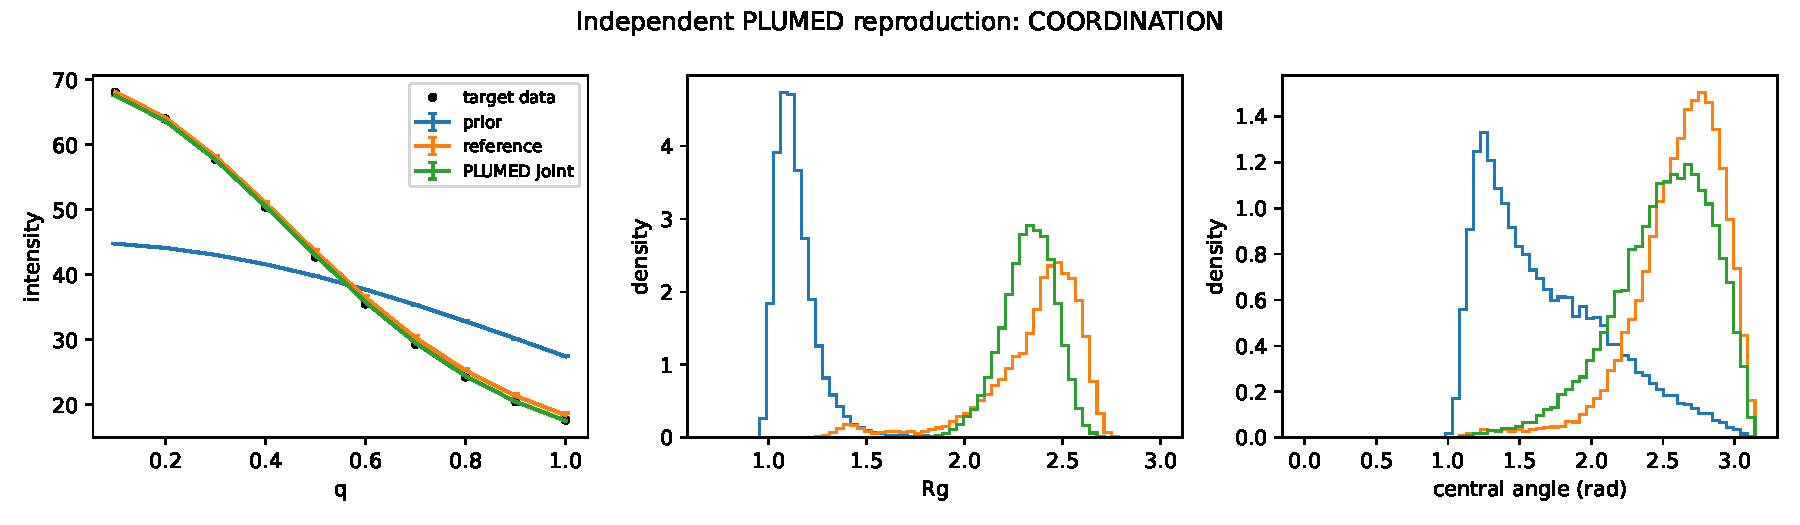
\includegraphics[width=\textwidth]{results/coordination-reproduction.pdf}
\caption{Independent PLUMED reproduction using COORDINATION: spectra, radius
of gyration and central bond angle. Spectral error bars are standard errors
across three independent frozen-production runs. The reference spectrum uses
the prescribed affine transformation; black points denote the original target.
Structural histograms pool the three runs.}
\end{figure}
\begin{figure}[ht]
\centering
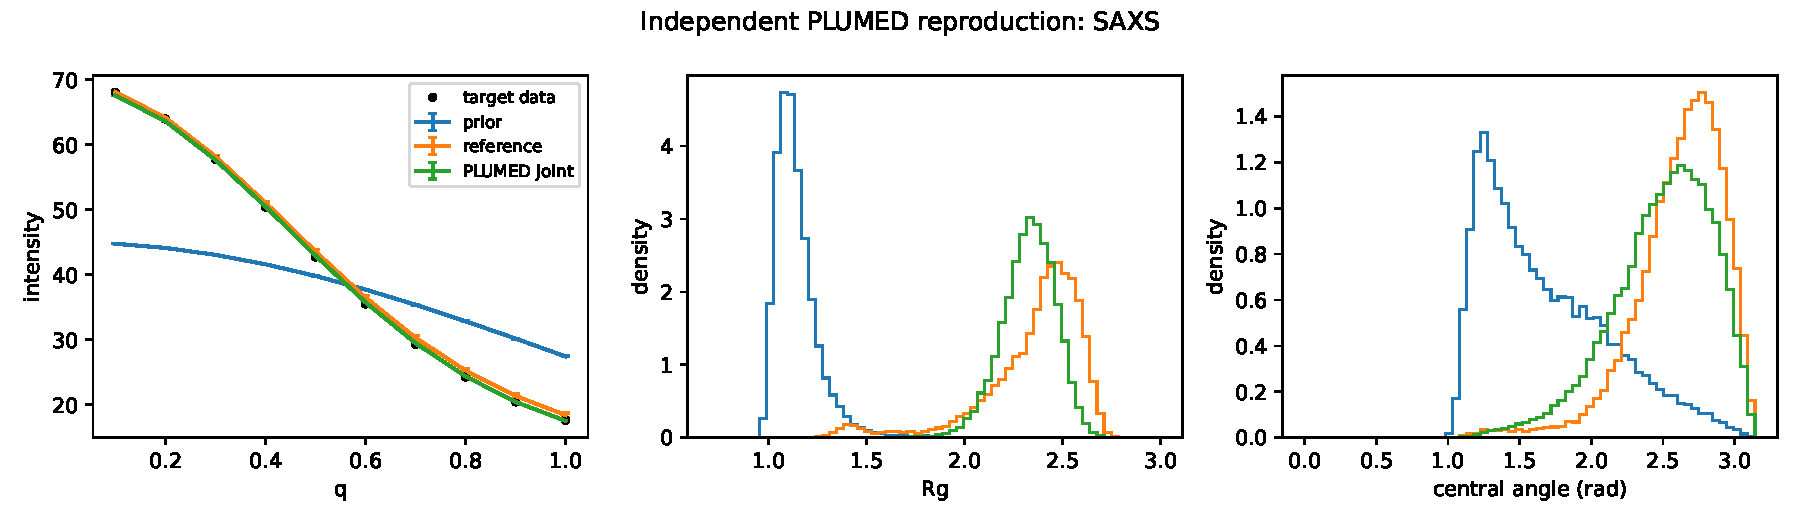
\includegraphics[width=\textwidth]{results/saxs-reproduction.pdf}
\caption{The corresponding independent PLUMED reproduction using SAXS.
Definitions and error bars are as in the preceding figure.}
\end{figure}
